\documentclass[11pt,a4paper]{article}

\usepackage[polish]{babel}
\usepackage[utf8]{inputenc}
\usepackage{polski}
\usepackage[T1]{fontenc}
\usepackage{indentfirst}
\usepackage{wrapfig}    % for wrapping figures, tables
\usepackage{isotope}
\usepackage{hyperref}
\usepackage{amsmath}
\usepackage{amssymb}
\usepackage{bm}
\usepackage{gensymb}
\usepackage{epsfig}
\usepackage{graphics}
\usepackage[shortlabels]{enumitem}
\usepackage{xspace}
\xspaceaddexceptions{[]\{\}}

%\def\hidesolutions{}  %← show solutions. Comment out to show solutions

%
%
%fixpagesize
\pagestyle{empty}
\addtolength{\textwidth}{4cm}
\addtolength{\textheight}{6cm}
\addtolength{\evensidemargin}{-3cm}
\addtolength{\oddsidemargin}{-2cm}
\addtolength{\topmargin}{-3cm}
\parindent=0cm

%
%
% Changes figure placing algorithm
\renewcommand{\topfraction}{1}       % maximal fraction of a page allowed for figures
\renewcommand{\textfraction}{0.15}   % minimal number of text for figure-text shared pages
\renewcommand{\floatpagefraction}{0.95} % if two above does not help, this could do the job 
                                        % must be: floatpagefraction < topfraction !!!!
\renewcommand{\textfraction}{0} % minimum fraction of page, which must be  devoted to text
\renewcommand{\topfraction}{1}  % maximum fraction at top, which can be occupied whit floats
\setcounter{totalnumber}{400}   % increase the number of floats for one page
\setcounter{topnumber}{200}     % at all/top/bottom.
\setcounter{bottomnumber}{200}  %

%
%
%small distance in list/item/enum for enumitem package
\setlist[itemize,enumerate]{topsep=0em}
\setlist{noitemsep}

%Nuclear notations: usage \nucl{235}{92}{U}. Math mode optional
\newcommand{\nucl}[3]{\ensuremath{
  \phantom{\ensuremath{^{#1}_{#2}}}
  \llap{\ensuremath{^{#1}}}
  \llap{\ensuremath{_{\rule{0pt}{.75em}#2}}}
  \mbox{#3} } 
} 

\newcounter{zadanie}\newcommand{\zadanie}[1][]{\addtocounter{zadanie}{1} ~\\  {\bf \emph{Exercise \arabic{zadanie} #1 }} \\}
\newcounter{zaddom}\newcommand{\zaddom}[1][]{\addtocounter{zaddom}{1} ~\\  {\bf \emph{Homework \arabic{zaddom} #1 }} \\}

%dynamic solutions hiding
\usepackage{comment}

\newif\ifhidesolutions
\ifdefined\hidesolutions
  \hidesolutionstrue
\else
  \hidesolutionsfalse
\fi

\ifhidesolutions
  \excludecomment{solution}
\else
  \newenvironment{solution}{\vspace{1cm} \par\textbf{Solution.} \vspace{1cm}}{}
\fi
%%%%%%%%%%%%%%%%%%%%%%%%%%%%%%%%%%%%%%%%%%
\begin{document}         

%%%%%%%%%%%%%%%%%%%%%%%%%%%%%%%%%%%%%%%%%%%%%%%%%%%%%
\begin{centering}
  {\bf {\Large
 Introduction to Experimental Particle Physics I \\
  Set I: Reminder of the basics
  }} \\  
\end{centering}

\vspace{1cm}
%%%%%%%%%%%%%%%%%%%%%%%%%%%%%%%%%%%%%%%%%%%%%%%%%%%%%%%
\zadanie[Physical constants]

Please calculate numerical values of the following physical constants:
\begin{itemize}
\item $\hbar c$ in MeV$\cdot$fm units    
\item $\alpha = \frac{e^{2}}{4 \pi \epsilon_0 \hbar c}$
\end{itemize} 

\vspace{0.2cm}

using values from CODATA 2022:
\begin{itemize}
\item $h = 6.626 \times 10^{-34}\,\mathrm{J\,s}$
\item $c = 2.998 \times 10^8\,\mathrm{m/s}$
\item $\mathrm{e} = 1.602 \times 10^{-19}\,\mathrm{C}$
\item $\epsilon_0 = 8.854 \times 10^{-12}\,\mathrm{F/m}$
\end{itemize}

\begin{solution}

\begin{align*}
\hbar c &= \frac{h c}{2\pi} = \frac{(6.626 \times 10^{-34}\,\mathrm{J\,s})(2.998 \times 10^8\,\mathrm{m/s})}{2\pi} \\
&= \frac{1.986 \times 10^{-25}\,\mathrm{J\,m}}{2\pi} = 3.161 \times 10^{-26}\,\mathrm{J\,m} = \\
&= 3.161 \times 10^{-26} \times \frac{1}{1.602 \times 10^{-19}} \times \frac{1}{10^{-15}}  \,\mathrm{eV\,fm} = 197.3 \times 10^{6}\,\mathrm{eV\,fm} = \\
& = 197.3\,\mathrm{MeV\,fm}
\end{align*}


Fine structure constant $\alpha$:
\begin{align*}
\alpha &= \frac{e^{2}}{4 \pi \epsilon_0 \hbar c} = \frac{(1.602 \times 10^{-19}\,\mathrm{C})^{2}}{4 \pi (8.854 \times 10^{-
12}\,\mathrm{F/m}) (3.161 \times 10^{-26}\,\mathrm{J\,m})} = \\
&= \frac{2.566 \times 10^{-38}\,\mathrm{C^{2}}}{3.517 \times 10^{-36}\,\mathrm{C^{2}/J} } = 0.0073 \approx \frac{1}{137}
\end{align*}


\end{solution}
%%%%%%%%%%%%%%%%%%%%%%%%%%%%%%%%%%%%%%%%%%%%%%%%%%%%%%%
%%%%%%%%%%%%%%%%%%%%%%%%%%%%%%%%%%%%%%%%%%%%%%%%%%%%%%%
\zadanie[Rutherford backscattering]

Please calculate cross section for backscattering: $\theta = \pi \pm 5^\circ$ of 
$\alpha$ particles with energy $E_\alpha = 5.3$ MeV
on a gold foil. Use nonrelativistic Rutherford formula, taking into account
the nucleus recoil. The gold nucleus has charge $Z=79$ and mass $M = 197$ u. 
Alpha particle has mass $m_\alpha = 4$ u. Use, and justify approximation for 
the Rutherford formula angle dependency.

\vspace{0.2cm}

{\bf Hint:} Recall correspondence between total two body kinetic energy 
in the center of mass frame and in the relative motion frame 

\begin{solution}

Rutherford formula for scattering of $\alpha$ particles on a nucleus with 
charge $Z$ in the center of mass frame is given by:
\begin{align*}
\frac{d\sigma}{d\Omega} = 
\left( \frac{Z e^2}{4\pi \epsilon_0} \right)^2 \frac{1}{(4 E^{*}_\alpha \sin^2(\theta/2))^2}
\end{align*}

Relation between energy in the nucleus rest frame $E_\alpha$ - 
corresponding to kinetic energy of relative motion of projectile and target -
and the center of mass frame $E_\alpha^{*}$ is given by:

\begin{align*}
E_\alpha^{*} = \frac{\mu v_{relative}^{2}}{2} = 
\frac{\mu}{m_\alpha} \frac{v_{relative}^{2}}{2 m_\alpha} =
|| v^{LAB}_{nucleus}=0: v_{relative} = v_{LAB} || = \\
\frac{\mu}{m_\alpha} E^{LAB}_\alpha = \frac{M m_\alpha}{M + m_\alpha} \frac{1}{m_\alpha} E^{LAB}_\alpha =
\frac{M}{M + m_\alpha} E^{LAB}_\alpha = \frac{197}{197 + 4} \cdot 5.3 \text{ MeV} = 5.2 \text{ MeV}
\end{align*}

The normalisation factor in the Rutherford formula is given by:
\begin{align*}
\frac{Z e^2}{4\pi \epsilon_0} = Z \alpha \hbar c = 79 \cdot \frac{1}{137} \cdot 197.3 \text{ MeV fm} = 113.5~\text{MeV fm}
\end{align*}

Differential cross section at $\theta = \pi$ is given by:
\begin{align*}
\frac{d\sigma}{d\Omega} = 
\left( \frac{113.5~\text{MeV fm}}{4 \cdot 5.2~\text{MeV} \cdot \sin^2(\pi/2)} \right)^2 = 
\left( \frac{113.5~\text{MeV fm}}{20.8~\text{MeV}} \right)^2 = 
29.7~\text{fm}^2/\text{sr} = 
29.7 \times 10^{-28}~\text{m}^2/\text{sr} = 29.7~\text{b/sr}
\end{align*}

The cross section does not change significantly in the range $\theta = \pi \pm 5^\circ$:
\begin{align*}
    \frac{1}{\sin^4(\theta/2)} \Big|_{\theta = 175^\circ} = \frac{1}{\sin^4(87.5^\circ)} = 1.0006 \approx 1
\end{align*}

therefore we can approximate the cross section by:
\begin{align*}
    \sigma \approx \frac{d\sigma}{d\Omega}\Big|_{\theta = \pi} \Delta \Omega
\end{align*}


The solid angle corresponding to the backscattering range is given by:
\begin{align*}
\Delta \Omega = \int d\Omega = 
\int_{\phi=0}^{2\pi} d\phi \int_{\theta=175^\circ}^{180^\circ} \sin(\theta) d\theta
= 2 \pi \int_{\theta=175^\circ}^{180^\circ} \sin(\theta) d\theta =\\
2 \pi (\cos(175^\circ) - \cos(180^\circ)) = 2 \pi (0.996 - 1)
= 2 \pi \cdot 0.0038 = 0.0239~\text{sr}
\end{align*}

Final value is:
\begin{align*}
\sigma = 29.7~\text{b/sr} \cdot 0.0239~\text{sr} = 0.71~\text{b}
\end{align*}

\newpage
\end{solution}
%%%%%%%%%%%%%%%%%%%%%%%%%%%%%%%%%%%%%%%%%%%%%%%%%%%%%%%%%%%
%%%%%%%%%%%%%%%%%%%%%%%%%%%%%%%%%%%%%%%%%%%%%%%%%%%%%%%%%%%
\zadanie[Yukawa pion mass estimation]

Assume that the interaction, that binds nucleons in the nucleus, 
is mediated by a $\pi$ particle of mass $m_\pi$. The mediation is realized 
by creation, and exchange of a particle "from vacuum" for a short period of time,
in accordance with the energy and time uncertainty relation:
\begin{align*}
\Delta E \cdot \Delta t \sim \hbar
\end{align*}

Estimate the mass of the $\pi$ particle.
Assuming the range of the nuclear force to be $r_0 = 2 \cdot 10^{-15}$ m, 
and energy is given by the mass of the $\pi$ particle, $\Delta E = m_\pi c^2$,

\begin{solution}

Let's simply put the values from the problem into the uncertainty relation.
Time is given by the time needed for the particle to travel the distance $r_0$ at 
the speed of light $c$:

\begin{align*}
& \Delta E \cdot \Delta t = m_\pi c^2 \cdot \frac{r_0}{c} \approx \hbar \to 
m_\pi c^{2} \approx \frac{\hbar c}{r_0} = \frac{197~\text{MeV fm}}{2~\text{fm}} =
99~\text{MeV}
\end{align*}

\end{solution}
%%%%%%%%%%%%%%%%%%%%%%%%%%%%%%%%%%%%%%%%%%%%%%%%%%%%%%%%%%%
%%%%%%%%%%%%%%%%%%%%%%%%%%%%%%%%%%%%%%%%%%%%%%%%%%%%%%%%%%%
\zadanie[Neutrino hypothesis]

Find in the literature electron energy distribution in the $\beta$ decay.
Sketch the distribution and explain why the neutrino hypothesis was proposed.

\begin{solution}

The electron spectrum in the $\beta$ decay is continuous,
 which was unexpected, as the energy of the electron should be 
 discrete if only two particles were involved in the decay. 
 This led to the proposal of the neutrino hypothesis by Wolfgang Pauli, 
 suggesting that an additional particle (the neutrino) is emitted in the 
 decay, carrying away some of the energy and momentum, thus explaining 
 the continuous spectrum observed for the electrons.

\begin{figure}[h!]
\centering
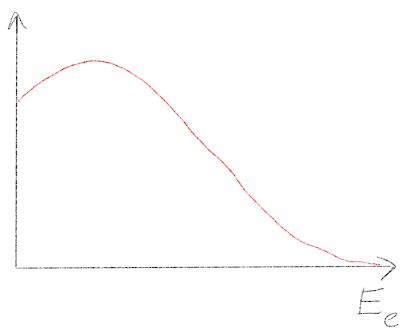
\includegraphics[width=0.6\textwidth]{e_spectrum_beta_decay.png}
\end{figure}


\end{solution}


\end{document}
